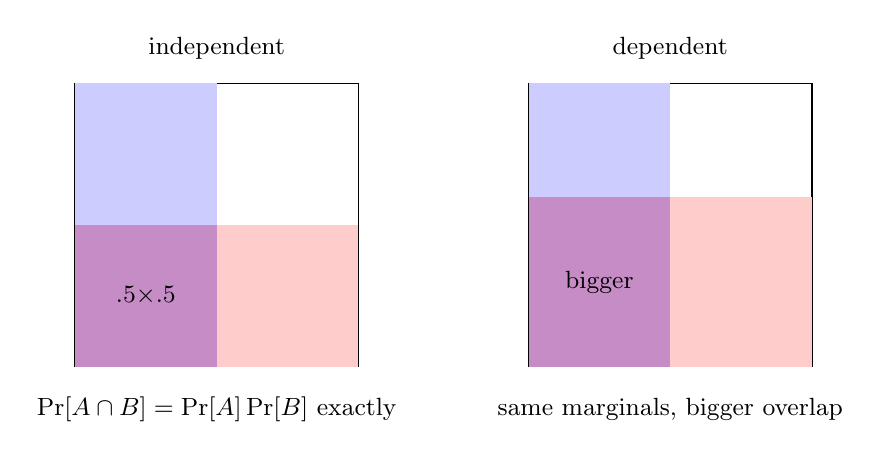
\begin{tikzpicture}[scale=0.9]
% independent: overlap = product; dependent: bigger overlap
\begin{scope}
\node at (2,4.5) {\small independent};
\draw (0,0) rectangle (4,4);
\fill[blue!20] (0,0) rectangle (2,4);
\fill[red!20] (0,0) rectangle (4,2);
\fill[violet!45] (0,0) rectangle (2,2);
\node at (1,1) {\small $.5{\times}.5$};
\node at (2,-0.6) {\small $\Pr[A\cap B]=\Pr[A]\Pr[B]$ exactly};
\end{scope}
\begin{scope}[xshift=6.4cm]
\node at (2,4.5) {\small dependent};
\draw (0,0) rectangle (4,4);
\fill[blue!20] (0,0) rectangle (2,4);
\fill[red!20] (0,0) rectangle (4,2.4);
\fill[violet!45] (0,0) rectangle (2,2.4);
\node at (1,1.2) {\small bigger};
\node at (2,-0.6) {\small same marginals, bigger overlap};
\end{scope}
\end{tikzpicture}
